Let us consider  we have a circle which passes through the point   $ \myvec { 1 \\ 2 \\	} $  and touches  x - axis at point  $ \myvec { r \\ 0 \\	} $ and y - axis  at $ \myvec { 0 \\ r \\ } $. Radius of the circle is $\vec{r}$ since it touches both axes. Hence we have 3 points which are :
\begin{align}
\vec{P_{1}} = \myvec{ 1 \\ 2 \\}
\end{align}
\begin{align}
\vec{p_{2}} = \myvec{ r \\ 0 \\}
\end{align}
\begin{align}
\vec{P_{3}} = \myvec{ 0 \\ r \\} \label{eq:solutions/4/2/6/2.3}
\end{align}

The general equation of circle is :
\begin{align}
\norm{\vec{x} - \vec{O}} = r
\end{align}

Substituting the given coordinates:
\begin{align}
\norm{  \vec{P_2} - \vec{O}}^{2} = r^{2} \label{eq:solutions/4/2/6/2.5}
\end{align}

\begin{align}
\norm{  \vec{ P_3} - \vec{O}}^{2} = r^{2} \label{eq:solutions/4/2/6/2.6}
\end{align}


\begin{align}
\norm{  \vec{ P_1} - \vec{O}}^{2} = r^{2} \label{eq:solutions/4/2/6/2.7}
\end{align}

From equation \ref{eq:solutions/4/2/6/2.5}, \ref{eq:solutions/4/2/6/2.6} and \ref{eq:solutions/4/2/6/2.7} we have 
%
%\begin{align}
%\norm{  \myvec{ r \\ 0 \\} - \vec{O}}^{2}  - \norm{ \myvec{ 1 \\ 2 \\}  - \vec{O}}^{2}   = 0 \label{eq:solutions/4/2/6/2.8}
%\end{align}
%
%\begin{align}
%\norm{ \myvec{ 0 \\ r \\} - \vec{O}}^{2}   - \norm{\myvec{ 1 \\ 2 \\} - \vec{O}}^{2}  = 0 \label{eq:solutions/4/2/6/2.9}
%\end{align}




\begin{align}
\norm{  \vec{ P_2} - \vec{O}}^{2}  - \norm{ \vec{P_1}  - \vec{O}}^{2}   = 0 \label{eq:solutions/4/2/6/2.8}
\end{align}
And,
\begin{align}
\norm{ \vec{ P_3} - \vec{O}}^{2}   - \norm{\vec{ P_1} - \vec{O}}^{2}  = 0 \label{eq:solutions/4/2/6/2.9}
\end{align}

 Simplifying   \ref{eq:solutions/4/2/6/2.8} and \ref{eq:solutions/4/2/6/2.9},
\begin{align}
\myvec{\vec{P_2} - \vec{O}}^T \myvec{\vec{P_2} - \vec{ O}} - \myvec{\vec{P_1} - \vec{O}}^T\myvec{\vec{P_1} - \vec{O}} = \vec{0} \label{eq:solutions/4/2/6/2.10}
\end{align}



\begin{align}
\implies \norm{\vec{P_2}}^2 - 2 \vec{P_2}^T\vec{O} - \norm{\vec{P_1}}^2 +2\vec{P_1}^T \vec{O}  = \vec{0} \label{eq:solutions/4/2/6/2.11}
\end{align}

 Substituting the value of $\norm{\vec{P_1}}$ and $\norm{\vec{P_2}}$ and other values then rearranging it, we get :
\begin{align}
\myvec{2 -2r & 4 \\}\myvec{O} = 5-r^2 \label{eq:solutions/4/2/6/2.12}
\end{align}





Similarly,

\begin{align}
\myvec{\vec{P_3} - \vec{O}}^T \myvec{\vec{P_3} - \vec{ O}} - \myvec{\vec{P_1} - \vec{O}}^T\myvec{\vec{P_1} - \vec{O}} = \vec{0} \label{eq:solutions/4/2/6/2.13}
\end{align}



\begin{align}
\implies \norm{\vec{P_3}}^2 - 2 \vec{P_3}^T\vec{O} - \norm{\vec{P_1}}^2 +2\vec{P_1}^T \vec{O}  = \vec{0} \label{eq:solutions/4/2/6/2.14}
\end{align}
Substituting the value of $\norm{\vec{P_1}}$ and $\norm{\vec{P_3}}$ and other values then  rearranging it, we get :

\begin{align}
\myvec{2  & 4 -2r \\}\myvec{O} = 5-r^2 \label{eq:solutions/4/2/6/2.15}
\end{align}















Combining \ref{eq:solutions/4/2/6/2.15} and \ref{eq:solutions/4/2/6/2.12}

\begin{align}
\myvec{2 - 2r  &  4 \\   2 & 4 - 2r \\} \myvec{O} = \myvec{5 - r^2 \\ 5 - r^2 \\} \label{eq:solutions/4/2/6/2.17}
\end{align}
Transforming the matrix into row-echelon form \\
\begin{align}
\myvec{2 - 2r  &  4 &  5 - r^2 \\   2 & 4 - 2r &  5 - r^2 \\}  \label{eq:solutions/4/2/6/2.18}
\end{align}

	\begin{align}
\myvec{
	2 - 2r & 4 & 5 - r^2 \\
	2 & 4 - 2r & 5 - r^2 \\
}
\xleftrightarrow[]{R1 \leftarrow \frac{R1}{2 - 2r} } \nonumber  \\
%
\myvec{
	1 & \frac{-2}{r-1} & \frac{r^2 - }{2\left( r - 1\right)} \\
	2 & 4 - 2r & 5 - r^2\\
}
\xleftrightarrow[]{R2 \leftarrow  R2 - 2R1 } \nonumber  \\
%
\myvec{
	1 & \frac{-2}{r - 1} & \frac{r^2 - 5}{2 \left( r - 1 \right)} \\
	0 & \frac{2r\left(r - 3 \right) }{ r - 1} & \frac{r \left(r^2 - 5 \right)}{r - 1}
}
\xleftrightarrow[]{R2 \leftarrow \left( \frac{1 - r}{ 2r \left( r - 3\right)}\right)R2 } \nonumber  \\
%	
\myvec{
	1 & \frac{-2}{r - 1} & \frac{r^2 - 5}{2 \left(r - 1\right)} \\
	0 & 1 & \frac{r^2 - 5}{2 \left(r - 3\right)}
}
\xleftrightarrow[]{R1 \leftarrow  R1 - \left( \frac{-2}{r - 1} \right)R2 } \nonumber   \\
\myvec{
	1 & 0 & \frac{r^2 - 5}{2 \left(r - 3\right)} \\
	0 & 1 & \frac{r^2 - 5}{2 \left(r - 3\right)}
}
\end{align}
So,
\begin{align}
\vec{O} = \myvec{ \frac{r^2 - 5}{2 \left(r - 3\right)} \\ \frac{r^2 - 5}{2 \left(r - 3\right)} \\} \label{eq:solutions/4/2/6/2.19}
\end{align}



Now subsituting the \ref{eq:solutions/4/2/6/2.3} in \ref{eq:solutions/4/2/6/2.7}, we have
\begin{align}
\norm{  \vec{ P_3} - \vec{O}}^{2} = r^{2} \label{eq:solutions/4/2/6/2.20}
\end{align}

Subsituting the value of $\vec{O}$ in \ref{eq:solutions/4/2/6/2.7} and simplify,
\begin{align}
\myvec{\vec{P_3} - \vec{O}}^T\myvec{\vec{P_3} - \vec{O}} = r^2 \label{eq:solutions/4/2/6/2.21}
\end{align}


\begin{align}
 \implies \norm{\vec{P_3}}^2 - \vec{P_3}^T\vec{O}  -  \vec{P_3} \vec{O}^T +\norm{\vec{O}}^2 = r^2 \label{eq:solutions/4/2/6/2.22.1}
\end{align}
Putting the values  of $\vec{O}$ from \ref{eq:solutions/4/2/6/2.19} and $\norm{\vec{P_3}}^2$

\begin{align}
\implies - \vec{P_3}^T\vec{O}  -  \vec{P_3} \vec{O}^T    = -  \norm{\vec{O}}^2 \label{eq:solutions/4/2/6/2.22.22}
\end{align}



\begin{align}
\implies - \myvec{0 \\ r}^T\myvec{ \frac{r^2 - 5}{2 \left(r - 3\right)} \\ \frac{r^2 - 5}{2 \left(r - 3\right)} \\}  -  \myvec{0 \\ r} \myvec{ \frac{r^2 - 5}{2 \left(r - 3\right)} \\ \frac{r^2 - 5}{2 \left(r - 3\right)} \\}^T    = -  \norm{\vec{O}}^2 \label{eq:solutions/4/2/6/2.22.2}
\end{align}

Subsituting the value of $\norm{\vec{O}}^2$ and simplify it,
\begin{align}
\implies 2r \left( \frac{r^2 - 5}{2 \left(r - 3\right)} \right) = 2 \left( \frac{r^2 - 5}{2 \left(r - 3\right)} \right)^2 
\end{align}




\begin{figure}[htb!]	
	\centering	
	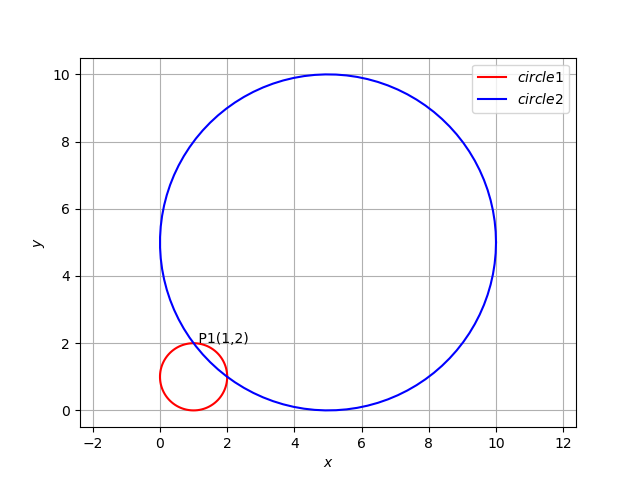
\includegraphics[width=\columnwidth]{./solutions/4/2/6/Circle.png}	
	\caption{Two circles passing through a common point}
	\label{eq:solutions/4/2/6/fig1}	
\end{figure}

\begin{align}
 \implies r  =  \frac{r^2 - 5}{2 \left(r - 3\right)} 
\end{align}


\begin{align}
\implies r^2 - 6r +5 = 0
\end{align}


\begin{align}
\implies \left( r -1\right) \left( r- 5\right) = 0
\end{align}

\begin{align}
\implies r = 1, r = 5.
\end{align}

Hence,
\begin{align}
\vec{O_1} = \myvec{5 \\ 5 \\} \text{and,}  \vec{O_2} = \myvec{1 \\ 1 \\}
\end{align}

Hence equation of circles are :
\begin{align}
\norm{\vec{x} - \myvec{5 \\ 5 \\}} = 5
\end{align}
And,
\begin{align}
\norm{\vec{x} - \myvec{1 \\ 1 \\}} = 1
\end{align}

